%--------------------------------------------------------------------
%--------------------------------------------------------------------
% Formato para los talleres del curso de Herramientas Computacionales
% Universidad de los Andes
%--------------------------------------------------------------------
%--------------------------------------------------------------------

\documentclass[11pt,letterpaper]{exam}
\usepackage[utf8]{inputenc}
\usepackage[spanish]{babel}
\usepackage{graphicx}
\usepackage{mdframed}
\usepackage{tabularx}
\usepackage[absolute]{textpos} % Para poner una imagen completa en la portada
\usepackage{multirow}
\mdfdefinestyle{mystyle}{leftmargin=1cm,rightmargin=1cm,linecolor=red}
\usepackage{float}
\usepackage{hyperref}
\usepackage{xcolor}
\decimalpoint
\hypersetup{colorlinks=false,linkbordercolor=red,linkcolor=green,pdfborderstyle={/S/U/W 1}}

%\usepackage{pst-barcode}
%\usepackage{auto-pst-pdf}

\newcommand{\base}[1]{\underline{\hspace{#1}}}
\boxedpoints
\pointname{ pt}
%\extrawidth{0.75in}
%\extrafootheight{-0.5in}
\extraheadheight{-0.15in}
%\pagestyle{head}

%\noprintanswers
%\printanswers
\renewcommand{\solutiontitle}{}
\SolutionEmphasis{\color{blue}}

\usepackage{upquote,textcomp}
\newcommand\upquote[1]{\textquotesingle#1\textquotesingle} % To fix straight quotes in verbatim

\begin{document}
\begin{center}
{\Large Herramientas Computacionales} \\
Taller 11 - \textsc{Python}: modelos computacionales sencillos \\
{\small \it Abril de 2015}
\end{center}

\begin{textblock*}{40mm}(10mm,20mm)
  
\includegraphics[width=3cm]{logoUniandes.png}
\end{textblock*}

\begin{textblock*}{40mm}(161mm,20mm)
  
\includegraphics[width=3cm]{logoUniandes.png}
\end{textblock*}

\vspace{1cm}

La solución de este taller debe ser presentada en un solo archivo (Notebook de iPython) con nombre \verb+NombreApellido_HW11.ipynb+. Puede trabajarse en grupos de máximo tres estudiantes.

\begin{center}
	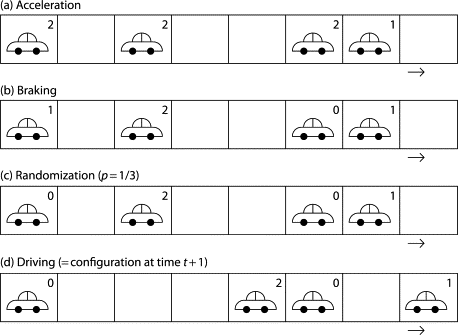
\includegraphics[width=0.6\textwidth]{ejemplo.png}
\end{center}

\begin{questions}

\question[100] En este taller vamos a simular el comportamiento del tráfico de carros en una calle circular de un solo carril y con una velocidad máxima $v_{max} = 5$, con un modelo llamado ``Modelo de Nagel-Schreckenberg para el tráfico''. En este modelo la vía está dividida en un número finito de espacios, en nuestro caso $1000$ espacios, y en cada uno de estos espacios cabe exactamente un carro. Vamos a tener $k$ carros en la vía, los cuales inicialmente van a estar distribuidos aleatoriamente sobre la misma. Cada carro comienza con una velocidad $v = 0$ y en cada paso de la simulación los carros avanzan $v$ espacios sobre la vía. Cada etapa de la simulación consiste en cuatro pasos que deben hacerse para todos los carros en paralelo. Esto quiere decir que no se debe mover ningún carro hasta que se hayan actualizado todas las velocidades. Los cuatro pasos son los siguientes: 

\begin{enumerate}
\item Si la velocidad es menor a la velocidad máxima, se aumenta la velocidad en una unidad. La gente siempre quiere ir más rápido. 
\begin{equation}
v \leftarrow min(v+1,v_{max})
\end{equation}
\item Se mira la distancia con el carro del frente. Si dicha distancia es $d$ y la velocidad del carro es mayor o igual que $d$, entonces se cambia la velocidad por $d-1$ para evitar colisiones. 
\begin{equation}
v \leftarrow min(v,d-1)
\end{equation}
\item Si la velocidad es positiva, entonces, con una probabilidad $p=1/3$, se reduce la velocidad en una unidad. Esto introduce el factor humano (aleatorio).
\begin{equation}
v \leftarrow max(0,v-1) \hspace{0.6cm} con \hspace{0.2cm} probabilidad \hspace{0.2cm} p
\end{equation}
\item En el cuarto paso todos los carros se mueven una distancia $v$. Así finaliza cada etapa de la simulación. 
\begin{equation}
x \leftarrow x+v
\end{equation}
\end{enumerate}

Para tener en cuenta que la vía es circular use aritmética módulo 1000 para las posiciones.

En la figura de arriba se muestra una etapa de la simulación \footnote{Andreas Schadschneider, Debashish Chowdhury and Katsuhiro Nishinari, Chapter Seven - Vehicular Traffic II: The Nagel–Schreckenberg Model, In Stochastic Transport in Complex Systems, edited by Andreas Schadschneider, Debashish Chowdhury and Katsuhiro Nishinari, Elsevier, Amsterdam, 2011, Pages 243-279, ISBN 9780444528537, http://dx.doi.org/10.1016/B978-0-444-52853-7.00007-5.
	(http://www.sciencedirect.com/science/article/pii/B9780444528537000075)} para una vía de $8$ espacios. En la parte superior derecha se muestra la velocidad, y cada línea del diagrama es cada uno de los 4 pasos de la simulación.


\begin{parts}
	\part[70] Construya una función llamada \verb+nagel+ que reciba como parámetro $k$ el número de carros en la vía y devuelva una matriz de tamaño $1000 \times 1000$ en donde cada renglón de la matriz tenga el estado de la vía al terminar cada etapa de la simulación. El estado de la vía está representado por una secuencia de ceros y unos donde $0$ representa un espacio vacío y $1$ un espacio ocupado. 
	
	Utilice un par de arreglos de tamaño $k$ para guardar las posiciones $x$ y velocidades $v$ y construya una función llamada \verb+makeroad+ que reciba el array con las posiciones y que entregue el estado de la vía. Abajo se muestra un ejemplo de la relación entre el arreglo con las posiciones y el estado de la vía para una simulación con una carretera de longitud 10 con 5 carros.
	
	\begin{tabular}{ |c|c|c|c|c| }
	\hline
  	2 & 3 & 6 & 7 & 0 \\
	\hline
	\end{tabular} (las posiciones)
	
	\begin{tabular}{ |c|c|c|c|c|c|c|c|c|c| }
	\hline
  	1 & 0 & 1 & 1 & 0 & 0 & 1 & 1 & 0 & 0 \\
	\hline
	\end{tabular} (la vía)
	
	Una vez tenga la función, ejecútela con $k=150$, y visualice el resultado para obtener algo similar a lo mostrado a continuación.

	\begin{center}
		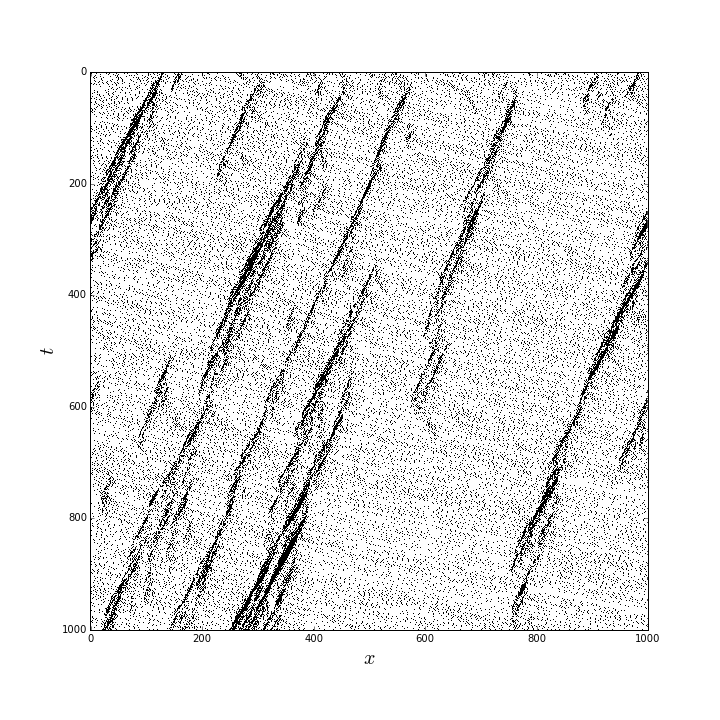
\includegraphics[width=0.9\textwidth]{trancones.png}
	\end{center}
	
	\part[30] Ahora construya una función llamada \verb+totaldistance+ que reciba el número $k$ de carros en la vía y entregue la distancia total recorrida por todos ellos en las 1000 iteraciones de la simulación. La distancia recorrida en cada etapa de la simulación es igual a la suma de todas las velocidades después de ejecutar el tercer paso.
	
	Luego use la función para calcular la distancia total para valores de k entre $10$ y $990$ en saltos de $10$. Haga una gráfica de la distancia total recorrida contra $k$. Aproximadamente, ¿para qué valor de $k$ se recorre la distancia total máxima? Comente los resultados.
	
	\begin{center}
			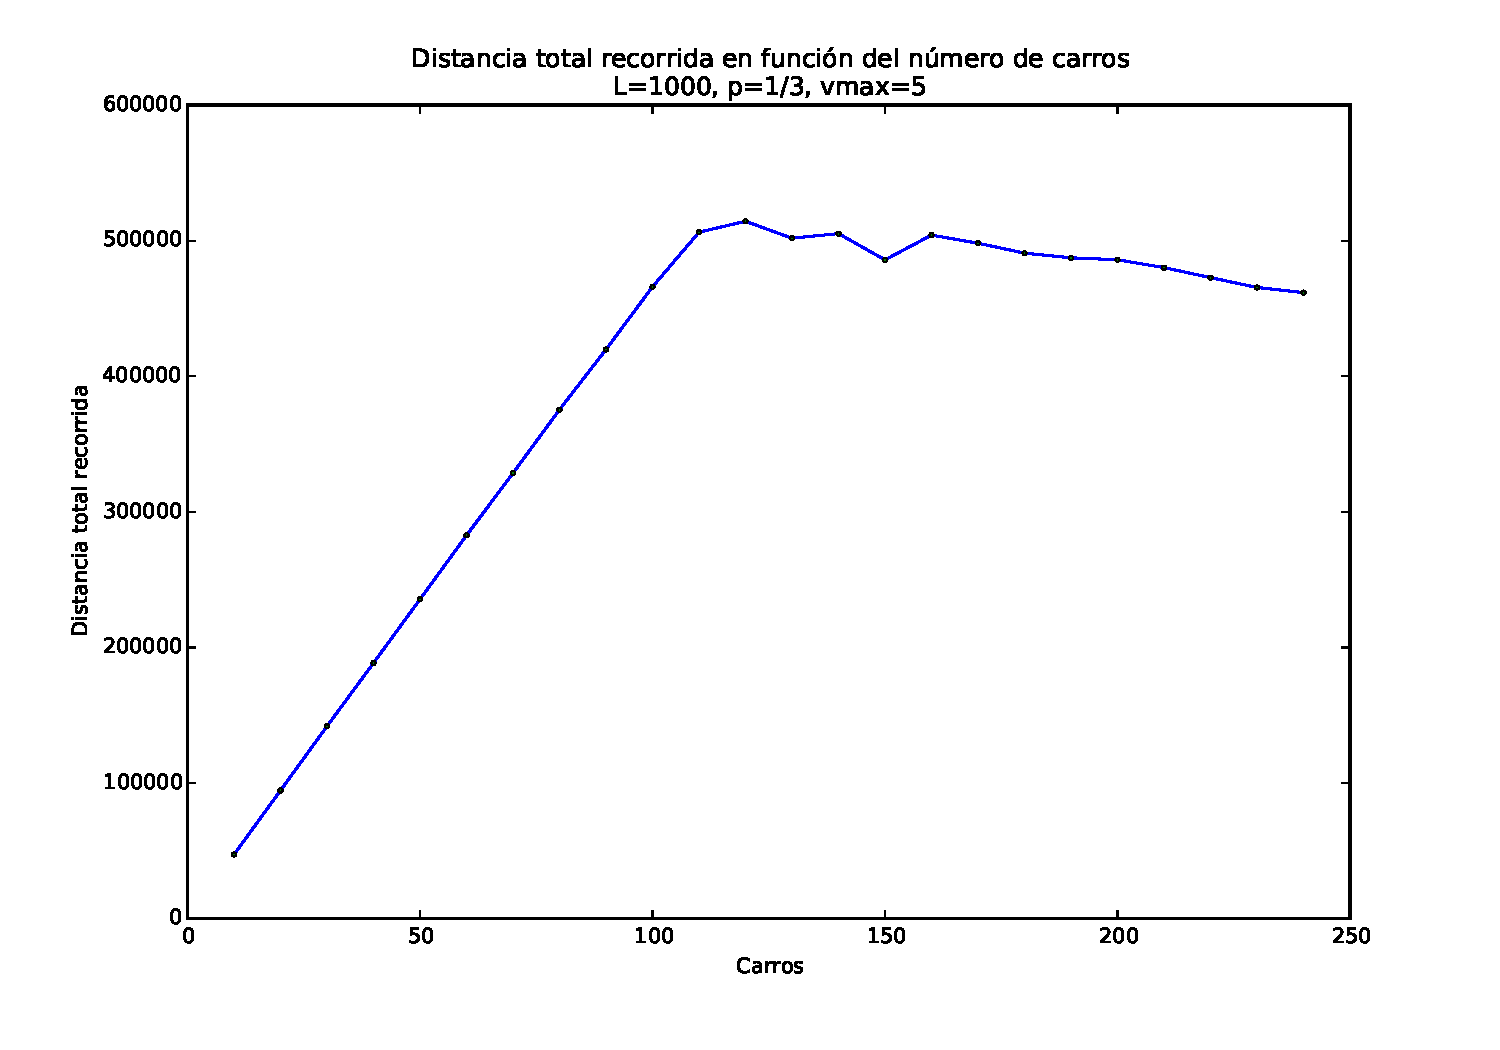
\includegraphics[width=0.95\textwidth]{flujo.pdf}
	\end{center}
	
\end{parts}

\end{questions}
\end{document}
